\chapter{Tangent Spaces}
  \section{Curves and Functions on a Manifold}
    \begin{definition}[Curve on a Manifold]
      A (parametrized) curve $\sigma$ on a m-dimensional manifold
      $\mathcal{M}$ is an injective map from $I\subset \mathbb{R}$ into
      $\mathcal{M}$ by:
      \begin{equation*}
        t\in I \rightarrow \sigma(t) \in \mathcal{M}
      \end{equation*}
    \end{definition}
      The curve is also said to be differentiable if the map $\sigma$ is
      differentiable.
    \begin{definition}[Differentiable Curve on a Manifold]
      The idea of $\sigma$ being differentiable is defined as follows:
      Consider a chart $(U, \phi)$ that covers the entire curve, i.e
      $\sigma(I) \subset U$. Then, $\sigma$ being differentiable is defined
      as the map $\bar{\sigma} \equiv \phi \circ \sigma$ from $I$ to
      $\mathbb{R}^m$ being differentiable.

      Note that $\bar{\sigma}(t) = \left(x^1(t),...x^m(t)\right)$, thus
      $\bar{\sigma}$ being differentiable means that the $m$ coordinate
      functions ${x^i(t)}$ are differentiable with respect to $t$. 

      Note also that the differentiability of $\sigma$ is coordinate
      independent, as can be easily proved by considering another chart
      $(V,\psi)$ that covers the entire curve, and noting that if $\phi
      \circ \sigma$ is differentiable, then so is $\psi \circ \sigma$
      because:
      \begin{equation}
        \label{eqn: cheap trick coordinate independence}
        \psi \circ \sigma = \underbrace{\psi \circ \phi^{-1}}_{\in C^k}
        \circ  \, \, \phi \circ \sigma
      \end{equation}
    \end{definition}
    \begin{remark}
      Equation~\ref{eqn: cheap trick coordinate independence} is an example
      of a really useful trick, where we insert an identity map $\phi^{-1}
      \circ \phi$ or $\phi \circ \phi^{-1}$ to show that certain things are
      independent of the chart chosen. In fact, we have seen something like
      this in section~\ref{sec: Diffeomorphism}. We will use this trick
      frequently, but from now on, we will not show the explicit calculation, but only make a brief comment.
    \end{remark}
    \begin{definition}[Function on a Manifold]
      A function $f$ on a manifold $\mathcal{M}$ is the map $f:\mathcal{M}
      \rightarrow \mathbb{R}$.
    \end{definition}
    \begin{definition}[$C^r$Function on a Manifold]
      A function $f$ on a manifold $\mathcal{M}$ is said to be $C^r$ at $p
      \in \mathcal{M}$ if in a chart $(U,\phi)$ such that $p\in U$,
      $\bar{f} \equiv f \circ \phi^{-1}$ is a $C^r$ function from
      $\mathbb{R^m}$ to $\mathbb{R}$.

      Note that the above defintion can be shown to be independent of the
      choice of chart $(U,\phi)$; we can consider another chart $(V, \psi)$
      and do the insertion of identity trick as was done in
      equation~\ref{eqn: cheap trick coordinate independence}.

      If $f$ is $C^r \,\, \forall p \in \mathcal{M}$, then we say that $f \in
      C^r(\mathcal{M})$, or that $f$ is a $C^r$ function on the manifold
      $\mathcal{M}$.
    \end{definition}
    \subsection{Useful notation: Overbar}
      The astute reader might have noticed by now that we have been quite
      consistent in our notation, in where we place an overbar.
      Specifically, for some chart $(U,\phi)$ we have done:
      \begin{itemize}
        \item{$f:\mathcal{M}\rightarrow \mathbb{R}$ leads to $\bar{f} \equiv f \circ \phi:\mathbb{R}^m \rightarrow \mathbb{R}$}
        \item{$\sigma:I \subset \mathbb{R} \rightarrow \mathcal{M}$ leads to
        $\bar{\sigma}\equiv \phi \circ \sigma: \mathbb{R} \rightarrow \mathbb{R}^m$}
      \end{itemize}
      Thus, for any map that involves a manifold $\mathcal{M}$, we shall
      use the overbar to denote its representation in some local coordinate
      system (i.e, in some chart). Some examples (including those which we will see later):
      \begin{itemize}
        \item{$f:\mathcal{M}\rightarrow \mathcal{N}$ leads to $\bar{f} =
        \phi^{-1}\circ f \circ \psi: \mathbb{R}^m \rightarrow \mathbb{R}^n$
        where $(U,\phi)$ is some chart in $M$, $(V,\psi)$ is some chart in
        $N$.}
        \item{$X: C^\infty(\mathcal{M})\rightarrow C^\infty(\mathcal{M})$
        leads to $\bar{X}:C^\infty(\mathbb{R}^m)\rightarrow
        C^\infty(\mathbb{R}^m)$}
      \end{itemize}
  \section{Tangent Vectors}
    \begin{definition}[Tangent Vector to a Curve]
      The tangent vector to a curve $\sigma$ at some point $p\in
      \mathcal{M}$ is defined:
      \begin{equation*}
        V^{\sigma}_{p}(f) = \frac{d}{dt}(f\circ\sigma)(t)\Bigr|_{t=0},
        \quad \sigma(0) = p
      \end{equation*}
      $\forall f \in C^k(\mathcal{M})$.
    \end{definition}
    Note that $V^{\sigma}_{p}(f)$ is a number. Now, there could be multiple
    curves with the same tangent vector; for example in $\mathbb{R}^2$, the
    curves $\sigma_1(t) = (t,e^t)$ and $\sigma_2(t) = (t, 1 + t)$ are
    tangent at $p = (1,1)\in \mathbb{R}^2$. Let's extend this idea to a
    general manifold $\mathcal{M}$.
    \begin{definition}[Two curves being tangent at $p\in \mathcal{M}$]
      \label{defn: two curves being tangent}
      Two curves on the manifold $\mathcal{M}$, $\sigma_1(t)$ and
      $\sigma_2(t)$, are said to be tangent at $\sigma_1(0) = \sigma_2(0) =
      p \in \mathcal{M}$ if for all $f \in C^k(\mathcal{M})$, the following
      holds:
      \begin{equation*}
        \frac{d}{dt}(f\circ \sigma_1)(t)\Bigr|_{t=0} = \frac{d}{dt}(f\circ
        \sigma_2)(t)\Bigr|_{t=0}
      \end{equation*}
    \end{definition}
    \begin{remark}
      The $\sigma_1(0) = \sigma_2(0) = p \in \mathcal{M}$ condition is just
      saying that the two curves must intersect. Without loss of
      generality, if $\sigma_1(t_1) = \sigma_2(t_1) = p \in \mathcal{M}$
      and $\frac{d}{dt}(f\circ \sigma_1)(t)|_{t=t_1} =
      \frac{d}{dt}(f\circ \sigma_2)(t)|_{t=t_1}$ for some $t_1\in
      \mathbb{R}$, then we can just do a change of variables $t = t + t_1$
      to recover our original definition. I.e, definition \ref{defn: two
      curves being tangent} is general enough.
    \end{remark}
    \begin{remark}
      In other words, two curves $\sigma_1(t)$ and $\sigma_2(t)$ are said
      to be tangent at $p\in \mathcal{M}$ if they have the same tangent
      vector at point $p\in \mathcal{M}$, i.e $V_p^{\sigma_1} =
      V_p^{\sigma_2}$. We will see what this means in more detail when we
      go into a local chart $(U,\phi)$.
    \end{remark}
    \subsection{Tangent vectors to a curve in a local chart $(U,\phi)$}
      This concept is very important and thus deserves a section of its
      own. Consider $p\in \mathcal{M}$, and a local chart $(U,\phi)$ around
      $p$, i.e $p\in U$. Consider also a curve $\sigma$ such that
      $\sigma(0)= p$.
      Then, we have:
        \begin{align*}
          V^{\sigma}_{p}(f) &= \frac{d}{dt}(f\circ\sigma)(t)\Bigr|_{t=0} \\
          &= \frac{d}{dt}(f\circ\phi^{-1}\circ \phi \circ
          \sigma)(t)\Bigr|_{t=0} \\
          &= \frac{d}{dt}(\bar{f}\circ\bar{\sigma})(t)\Bigr|_{t=0}
        \end{align*}
      where $\bar{\sigma}(t) = \left(x^1(t),...,x^m(t)\right)$ is a curve
      in $\mathbb{R}^m$, and $\bar{f}$ is a map from $\mathbb{R}^m$ to
      $\mathbb{R}$. Continuing with our calculation, we have:
        \begin{align*}
          V^{\sigma}_{p}(f)
          &=\frac{d}{dt}(\bar{f}\circ\bar{\sigma})(t)\Bigr|_{t=0} \\
          &=\frac{d}{dt}\bar{f}(x^1(t),...,x^m(t))\Bigr|_{t=0}\\
          &=\frac{dx^i}{dt}\Bigr|_{t=0}\frac{\partial \bar{f}}{\partial
          x^i}\Bigr|_{\phi(p)} \\
          &=\frac{dx^i}{dt}\Bigr|_{t=0}\frac{\partial}{\partial x^i}(\bar{f})
        \end{align*}
      where in the last line, we write $\frac{\partial \bar{f}}{\partial
      x^i}\Bigr|_{\phi(p)}$ as $\frac{\partial \bar{f}}{\partial x^i}$ for
      ease of notation, as we will sometimes do in the future. Now, since
      the above calculations are true for all $f \in C^k(\mathcal{M})$, we
      have:
      \begin{equation}
        \label{eqn: tangent vector to a curve in local coords}
        V^{\sigma}_{p} \xrightarrow{\text{local chart}}
        \frac{dx^i}{dt}\Bigr|_{t=0}\frac{\partial}{\partial x^i}
      \end{equation}
      Equation~\ref{eqn: tangent vector to a curve in local coords} tells
      us what it means for two curves $\sigma_1(t)$ and $\sigma_2(t)$ to be
      tangent at $p\in\mathcal{M}$. In a local chart $(U,\phi)$,
      $\sigma_1(t)$ and $\sigma_2(t)$ are tangent at $p\in\mathcal{M}$ if and only if these two conditions hold:
      \begin{enumerate}
        \item{$\sigma_1(0) = \sigma_2(0) = p$}
        \item{\label{item: tangent condition}If we write $\bar{\sigma_1}(t)
        = \left(x^1(t),...,x^m(t)\right)$ and $\bar{\sigma_2}(t) =
        \left(x^{\prime 1}(t),...,x^{\prime m}(t)\right)$, then
        \begin{equation*}
          \frac{dx^i}{dt}\Bigr|_{t=0} = \frac{dx^{\prime i}}{dt}\Bigr|_{t=0}
        \end{equation*}}
        for all $i = 1,...,m$.
      \end{enumerate}
    By the way, it can be proven\footnote{Refer to Kuldip's tutorials, or
    Nakahara/Frankel} that if condition~\ref{item: tangent condition} is
    true in one local chart $(U,\phi)$, then it is true for all charts. 
    
    \subsection{Motivating the definition of a tangent vector at a point}
      So far, we have defined a tangent vector to a curve. However, the
      above calculation explicitly shows us that we cannot identify tangent
      vectors uniquely with curves, since there could be many different
      curves that give the same tangent vector.
      
      However, if we take the set of all curves that pass through a point
      $p\in \mathcal{M}$, and separate them into equivalence classes where
      the equivalence relation between two curves is that they are tangent
      at the point $p\in \mathcal{M}$, then we can uniquely identify
      different tangent vectors with different equivalence classes of
      curves. This is what we will do.

    \begin{definition}[Tangent Vector at a point $p \in \mathcal{M}$]
      \label{defn: Tangent vector at a point}
      A tangent vector at $p \in \mathcal{M}$, $V^{\sigma}_{p}$ is defined
      as \begin{equation*}
          V^{\sigma}_{p}(f) = \frac{d}{dt}(f\circ\sigma)(t)\Bigr|_{t=0},
          \quad \sigma(0) = p
        \end{equation*}
      $\forall f\in C^k(\mathcal{M})$, where $\sigma$ is any representative
      of an equivalence class of curves, denoted $[\sigma]_p$. The
      equivalence relation between two curves is that they are tangent at
      the point $p\in \mathcal{M}$.
    \end{definition}
    \begin{remark}
      Sometimes, we write $V^{\sigma}_{p} = [\sigma]_p$, i.e we identify
      the tangent vector directly with the equivalence class of curves that
      it is defined with. Recall: different equivalence class of curves
      $\implies$ different tangent vectors!

      In fact, we will do this a lot in this set of notes; this is a convention inherited from Kuldip.
    \end{remark}
    \subsection{Tangent vectors at a point $p\in\mathcal{M}$ in a local
    chart $(U,\phi)$}
      The local representation of a tangent vector at a point,
      $V^{\sigma}_{p}$, is exactly the same the local representation of a
      tangent vector to a curve, given in equation~\ref{eqn: tangent vector
      to a curve in local coords}. The only difference is that the term
      $\frac{dx^i}{dt}\Bigr|_{t=0}$ is now uniquely identified with an
      equivalence class of curves $[\sigma]_p$. Let's reproduce
      equation~\ref{eqn: tangent vector to a curve in local coords} here
      for convenience:
      \begin{equation*}
        V^{\sigma}_{p} \xrightarrow{\text{local chart}}
        \frac{dx^i}{dt}\Bigr|_{t=0}\frac{\partial}{\partial x^i}
      \end{equation*} Now, we can write $V^i \equiv
      \frac{dx^i}{dt}\Bigr|_{t=0}$, and call $V^i$ the components of the
      vector $V^{\sigma}_{p}$ in a local chart $(U,\phi)$. Then, we have:
      \begin{equation}
        \label{eqn: Tangent vector to a point local coord}
        V^{\sigma}_{p} \xrightarrow{\text{local chart}} V^i
        \frac{\partial}{\partial x^i} = V^i \partial_i
      \end{equation}
      From equation~\ref{eqn: Tangent vector to a point local coord}, we
      also see that $V^{\sigma}_{p}$ is associated with a directional
      derivative in a local coordinate chart. This is the breakthrough of
      modern differential geometry, to associate tangent vectors to a point
      in the manifold with a directional derivative in $\mathbb{R}^m$. Note
      that because $V^{\sigma}_{p}$ is associated with a directional
      derivative, we have the Leibniz product rule. We will revisit this idea again when we talk about derivations.

      Lastly, we shall call the $m$ objects $\{\partial_i\}_{i=1,...,m}$
      the coordinate basis vectors to the tangent space $T_p(\mathcal{M})$.
      But let's not get ahead of ourselves, and revisit this idea again
      later when we formally develop the tangent space.

      Note that from here on, whenever we say "tangent vector", we are
      referring to tangent vectors at a point. Also, from
      definiton~\ref{defn: Tangent vector at a point}, we see that a local
      chart is unnecessary to define a tangent vector; local charts are
      used just for our convenience, when we want to do computations.
    \subsection{Transformation properties of the components of a tangent
    vector when we switch local charts}
      Since tangent vectors exist independently of any local charts, lets
      see how the components of the tangent vector $V^\sigma_p$ in a local
      chart $(U,\phi)$ are related to the components in another local chart
      $(U^\prime, \phi^\prime)$.

      Consider $f\in C^k(\mathcal{M})$. Then, in the local chart
      $(U,\phi)$, we have:
      \begin{equation*}
        V^\sigma_p(f) = V^i \left(\frac{\partial}{\partial x^i}
        \bar{f}(x^1,...,x^m)\right)\Bigr|_{\phi(p)}
      \end{equation*}
      where $\bar{f} = f \circ \phi^{-1}$.
      On the other hand, in the other local chart $(U^\prime,\phi^\prime)$,
      we have:
      \begin{equation*}
        V^\sigma_p(f) = V^{\prime i} \left(\frac{\partial }{\partial x^{\prime
        i}}\bar{f^\prime}(x^{\prime 1},...,x^{\prime m})\right)\Bigr|_{\phi^\prime(p)}
      \end{equation*}
      where $\bar{f^\prime} = f \circ \phi^{\prime-1}$.
      Note that $\bar{f}(x^1,...,x^m) = \bar{f^\prime}(x^{\prime
      1},...,x^{\prime m}) = f(p)$.

      But $\phi^{\prime} \circ \phi^{-1}$, a map from $\phi(U\cap U^\prime)
      \subset \mathbb{R}^m$ to $\phi^\prime(U\cap U^\prime) \subset
      \mathbb{R}^m$, induces $m$ coordinate transformation functions
      $\left\{x^{\prime i}(x^1,...,x^m)\right\}_{i=1,...,m}$. Thus, using the chain rule, we have:
      \begin{align*}
        \left(\frac{\partial}{\partial x^i}
        \bar{f}(x^1,...,x^m)\right)\Bigr|_{\phi(p)} 
        &= \left(\frac{\partial}{\partial x^i} \bar{f^\prime}(x^{\prime
        1}(x^1,...,x^m),...,x^{\prime m}(x^1,...,x^m))\right)
        \Bigr|_{\phi(p)}\\
        &= \frac{\partial x^{\prime j}}{\partial x^i}\Bigr|_{\phi(p)}
        \left(\frac{\partial }{\partial x^{\prime
        j}}\bar{f^\prime}(x^{\prime 1},...,x^{\prime
        m})\right)\Bigr|_{\phi^\prime(p)}
      \end{align*}
      Thus, substituting the chain rule calculation above into the
      expression for $V_p^\sigma(f)$ in the local chart $(U,\phi)$, we
      have:
      \begin{equation*}
        V^\sigma_p(f) = V^i \frac{\partial x^{\prime j}}{\partial
          x^i}\Bigr|_{\phi(p)} \left(\frac{\partial }{\partial x^{\prime
          j}}\bar{f^\prime}(x^{\prime 1},...,x^{\prime
          m})\right)\Bigr|_{\phi^\prime(p)}
      \end{equation*}
      which, when we compare with the expression for $V_p^\sigma(f)$ in the
      local chart $(U^\prime,\phi^\prime)$, we get:
      \begin{equation}
        \label{eqn: Tangent vector component contravariant transformation}
        V^{\prime i} = V^i \frac{\partial x^{\prime j}}{\partial
        x^i}\Bigr|_{\phi(p)}
      \end{equation}
      Thus, we note that the components of the tangent vector in a local
      coordinate chart transforms contravariantly under a change of
      coordinates! This contravariant transformation is a direct
      consequence of the identification of tangent vectors with directional
      derivatives in a local coordinate chart.
    \subsection{Tangent vectors as derivations}
      From definiton~\ref{defn: Tangent vector at a point}, we see that
      $V_p^\sigma$ is really a map from $C^k(\mathcal{M}) \rightarrow
      \mathbb{R}$. In fact, since
      \[V_p^\sigma(f) = V^i \frac{\partial\bar{f}}{\partial x^i}\]
      in a local chart $(U,\phi)$, where $\bar{f} = f\circ \phi^{-1}$,we
      have the following few properties:
      \begin{enumerate}
        \item{$V_p^\sigma(f+g) = V_p^\sigma(f) + V_p^\sigma(g) \quad
        \forall f \in C^k(\mathcal{M})$}
        \item{$V_p^\sigma(\alpha f) = \alpha V_p^\sigma(f) \quad \forall
        \alpha\in\mathbb{R} \text{ and } \forall f \in C^k(\mathcal{M})$}
        \item{$V_p^\sigma(f\cdot g) = g(p)V_p^\sigma(f) + f(p)V_p^\sigma(g)
        \quad \forall f,g\in C^k(\mathcal{M})$}
      \end{enumerate}
      Thus, $V^\sigma_p$ is something we call a derivation, which is a
      fancy name for a generalised derivative operator that satisfies the
      three properties above (and especially Leibniz's product rule).
  \section{The Tangent Space \texorpdfstring{$T_p(\mathcal{M})$}{Tp(M)}}
    \subsection{Constructing the Tangent Space $T_p(\mathcal{M})$}
      Here, we want to show that the set of all tangent vectors at a point
      $p\in \mathcal{M}$, which we denote as $\{V_p^\sigma\}$, has a vector
      space structure. 

      To do so, we first need to define the addition between two tangent
      vectors $V^{\sigma_1}_p = [\sigma_1]$ and $V^{\sigma_2}_p =
      [\sigma_2]$. Since tangent vectors are identified uniquely with
      equivalence classes of curves, if we could take the two equivalence
      classes of curves and produce a third equivalence class of curves, then
      we would have produced another tangent vector. Note that it is possible
      for $[\sigma_1] = [\sigma_2]$, in which case our result will still be
      in the same equivalence class as $[\sigma_1]$ (i.e, adding of two
      parallel vectors will give a third parallel vector).

      In other words, given a two curves that pass through $\sigma_1$ and
      $\sigma_2$ that pass through $p \in \mathcal{M}$, we want a third curve
      $\sigma_3$ that passes through $p \in \mathcal{M}$ too. We will do so
      like this:
      \begin{enumerate}
        \item{Firstly, choose a local chart $(U,\phi)$ such that $p\in U$ and
        $\phi(p) = \vec{0}$, where $\vec{0}\in \mathbb{R}^m$.}
        \item{Secondly, make sure also that $\bar{\sigma_1}(0) =
        \bar{\sigma_2}(0) = \vec{0}$, where $\bar{\sigma_i} \equiv \phi \circ
        \sigma_i$.}
        \item{Since $\bar{\sigma_1}(t)$ and $\bar{\sigma_2}(t)$ are two
        curves in $\mathbb{R}^m$, and because $\mathbb{R}^m$ has a vector
        space structure, $\left(\bar{\sigma_1}(t) + \bar{\sigma_2}(t)\right)$
        is another curve in $\mathbb{R}^m$. Note that since
        $\left(\bar{\sigma_1}(0) + \bar{\sigma_2}(0)\right) = \vec{0} =
        \phi(p)$, this curve passes through $\phi(p)$.}
        \item{Since $\phi$ is a homeomorphism, $\phi^{-1}\circ
        \left(\bar{\sigma_1}(t) + \bar{\sigma_2}(t)\right)$ would be another
        curve in $\mathcal{M}$ that passes through $p$.}
      \end{enumerate}
      Thus, we shall define the addition operator between $V^{\sigma_1}_p$
      and $V^{\sigma_2}_p$ as follows:
      \begin{equation}
        \label{eqn: Tangent vector addition}
        V^{\sigma_1}_p + V^{\sigma_2}_p \equiv [\phi^{-1}\circ
        \left(\bar{\sigma_1}(t) + \bar{\sigma_2}(t)\right)]
      \end{equation}
      Next, we need to define the scalar multiplication of a tangent vector
      $V_p^\sigma$. We shall do so via:
      \begin{equation}
        \label{eqn: Tangent vector scalar multiplication}
        \alpha V^{\sigma}_p \equiv [\phi^{-1}\circ
        \left(\alpha\bar{\sigma}(t)\right)]
      \end{equation}
      In the cases of scalar multiplication, we have basiaclly mapped
      $\sigma(t)$ into $\mathbb{R}^m$ to give us a vector $\bar{\sigma}(t) \in
      \mathbb{R}^m$, then we multiplied $\alpha \in \mathbb{R}$ to
      $\bar{\sigma}(t)$ to give us another vector in $\mathbb{R}^m$, before mapping the result back to $\mathcal{M}$ through $\phi^{-1}$. This gives us another curve in $\mathcal{M}$ that passes through the point $p$.

      Now, to show that the equations~\ref{eqn: Tangent vector
      addition},\ref{eqn: Tangent vector scalar multiplication} do indeed
      endow the set $\{V_p^\sigma\}$ with a vector space structure, it suffices
      to show that:
      \begin{equation*}
        \left(\alpha V^{\sigma_1}_p+ \beta V^{\sigma_2}_p\right)(f)= \alpha
        V^{\sigma_1}_p(f) + \beta V^{\sigma_2}_p(f)
      \end{equation*}
      $\forall f\in C^k(\mathcal{M}),\,\,\forall \alpha,\beta \in \mathbb{R}$.
      \begin{proof}
        Let $\phi\circ\sigma_1 = \bar{\sigma_1}(t) =
        \left(x^1(t),...,x^m(t)\right)$, $\phi\circ\sigma_2 =
        \bar{\sigma_2}(t) = \left(y^1(t),...,y^m(t)\right)$ and $\bar{f} =
        f \circ \phi^{-1}$, where clearly $\bar{f}$ is a map from
        $\mathbb{R}^m$ to $\mathbb{R}$. By construction, $\bar{\sigma_1}(0)
        = \bar{\sigma_2}(0) = \phi(p) = \vec{0}$. We shall also define:
        \begin{align*}
          \alpha\bar{\sigma_1}(t) + \beta\bar{\sigma_2}(t) &= \alpha
          \left(x^1(t),...,x^m(t)\right) + \beta
          \left(y^1(t),...,y^m(t)\right) \\
          &\equiv (z^1(t),...,z^m(t))
        \end{align*}
        Now, 
        \begin{align*}
          \left(\alpha V^{\sigma_1}_p+ \beta V^{\sigma_2}_p\right)(f) 
          &= \frac{d}{dt}\big[\underbrace{f\circ\phi^{-1}}_{\bar{f}}\circ
          \left(\alpha\bar{\sigma_1}(t) +
          \beta\bar{\sigma_2}(t)\right)\big]\Bigr|_{t=0} \\
          &= \frac{d}{dt}\big[\bar{f}(z^1(t),...,z^m(t))\big] \\
          &= \frac{\partial}{\partial z^i}
          \bar{f}(z^1,...,z^m)\Bigr|_{\phi(p)} \frac{dz^i}{dt}\Bigr|_{t =
          0}\\
          &= \frac{\partial}{\partial z^i}
          \bar{f}(z^1,...,z^m)\Bigr|_{\vec{0}} \left(\alpha
          \frac{dx^i}{dt}\Bigr|_{t = 0} + \beta \frac{dy^i}{dt}\Bigr|_{t =
          0}\right) \\
          &= \alpha \frac{dx^i}{dt}\Bigr|_{t = 0}\frac{\partial}{\partial
          z^i} \bar{f}(z^1,...,z^m)\Bigr|_{\vec{0}} + \beta
          \frac{dy^i}{dt}\Bigr|_{t = 0}\frac{\partial}{\partial z^i}
          \bar{f}(z^1,...,z^m)\Bigr|_{\vec{0}} \\
          &= \alpha \frac{dx^i}{dt}\Bigr|_{t = 0}\frac{\partial}{\partial
          x^i} \bar{f}(x^1,...,x^m)\Bigr|_{\vec{0}} + \beta
          \frac{dy^i}{dt}\Bigr|_{t = 0}\frac{\partial}{\partial y^i}
          \bar{f}(y^1,...,y^m)\Bigr|_{\vec{0}} \\
          &= \alpha \frac{d}{dt}\big[f\circ\sigma_1\big]\Bigr|_{t=0} +
          \beta \frac{d}{dt}\big[f\circ\sigma_1\big]\Bigr|_{t=0} \\
          &= \alpha V^{\sigma_1}_p(f) + \beta V^{\sigma_2}_p(f)
        \end{align*}
        where to get from the 5th line of the proof to the 6th line, we do
        a renaming of variables.
      \end{proof}
      Thus, we see that the set $\{V_p^\sigma\}$ with the addition operator
      and the scalar multiplication operation defined in
      equations~\ref{eqn: Tangent vector addition}, \ref{eqn: Tangent vector
      scalar multiplication} does indeed have a (real) vector space
      structure, which we denote as $T_p(\mathcal{M})$.

    \subsection{Basis vectors of the Tangent Space $T_p(\mathcal{M})$}
      In a local coordinate chart $(U,\phi)$, we recall that we have:
      \[V^\sigma_p \xrightarrow{\text{local chart}} V^i
      \frac{\partial}{\partial x^i} \] 
      
      Now, since $T_p(\mathcal{M})$ has a vector space structure, we call
      the set of $m$ vectors $\{\frac{\partial}{\partial x^i}\}$ the
      coordinate basis\footnote{Since the coordinates $x^i$ are
      independent, the vectors in $\{\frac{\partial}{\partial x^i}\}$ are
      linearly independent} of the Tangent Space $T_p(\mathcal{M})$ (in a
      local chart). Coordinate basis means that these basis vectors
      $\frac{\partial}{\partial x^i}$are directly derived from the
      coordinates $x^i$.

      We can use a non-coordinate basis too; i.e our basis can be of the
      form:
      \[
        \underbrace{\left\{a^i\frac{\partial}{\partial x^i}, b^i\frac{\partial}{\partial
      x^i},... \right\}}_{m \text{ linearly independent vectors}}
      \]
      However, using a coordinate basis has many benefits\footnote{Kuldip
      didn't talk much about this, but Edward Teo talked about this
      more.}, which is why we will stick with a coordinate basis unless
      explicitly stated.
  \section{The push-forward map between Tangent Spaces}
    \label{sec: push forward between tangent spaces}
    If we have a differentiable map between two manifolds \[\mathcal{F}:
    \mathcal{M} \rightarrow \mathcal{N}\] at the point $p \in \mathcal{M}$,
    then this map induces a map between the tangent spaces
    $T_p(\mathcal{M})$ and $T_{\mathcal{F}(p)}(\mathcal{N})$
    \[\mathcal{F}_{*}:T_p(\mathcal{M}) \rightarrow
    T_{\mathcal{F}(p)}(\mathcal{N})\]
    The origins of this "push-forward" map will be obvious when we look at its definition.
    \begin{definition}[The Push-forward of a tangent vector]
      \label{defn: push-forward defn}
      If $\mathcal{F}: \mathcal{M} \rightarrow \mathcal{N}$ is a
      differentiable map at $p \in \mathcal{M}$ and $V_p^\sigma \equiv
      [\sigma]_p \in T_p(\mathcal{M})$, then the push-forward
      $\mathcal{F}_{*}(V_p^\sigma)$ in $T_{\mathcal{F}(p)}(\mathcal{N})$ is defined by 
      \[\mathcal{F}_{*}(V_p^\sigma) = [\mathcal{F} \circ
      \sigma]_{\mathcal{F}(p)}\]
      We can also write \[\mathcal{F}_{*}(V_p^\sigma) = W^{
      \sigma^\prime}_{\mathcal{F}(p)}\] where $\sigma^\prime = \mathcal{F}
      \circ \sigma$.
    \end{definition}
    \begin{remark}
      We can also consider a map $\mathcal{F}: \mathcal{M} \rightarrow
      \mathcal{M}$. In this case, $\mathcal{F}_{*}$ would be a map between
      the two tangent spaces of $\mathcal{M}$, i.e
      $\mathcal{F}_{*}:T_p(\mathcal{M}) \rightarrow
      T_{\mathcal{F}(p)}(\mathcal{N})$. We can also consider the case where
      $\mathcal{F}$ is a homeomorphism $\phi$.\footnote{A homeomorphism
      $\phi$ to $U\subset\mathbb{R}^n$ is a differentiable map. To see why,
      consider another chart $(V,\psi)$. Then, the condition for $\phi$ to
      be a differentiable map is that $\phi \circ \psi^{-1}$ is $C^k$,
      which is naturally satisfied by the definition of differentiable
      manifold.}
    \end{remark}
    To understand definiton~\ref{defn: push-forward defn}, suppose we have
    a curve $\sigma \subset \mathcal{M}$ passing through $p \in
    \mathcal{M}$. Then, the map $\mathcal{F}$ maps every point of $\sigma$
    to a curve $\mathcal{F} \circ \sigma \subset \mathcal{N}$, where
    $\mathcal{F} \circ \sigma$ is a curve passing through $\mathcal{F}(p)
    \in \mathcal{N}$. We can do this not only for $\sigma$, but for an
    entire equivalence class of curves
    \footnote{This is proven in one of Kuldip's tutorials. Essentially, we
    want to show that if two curves $\sigma_1(t)$ and $\sigma_2(t)$ belong
    in the same equivalence class $[\sigma]_p$ at the point
    $p\in\mathcal{M}$, then the two curves $\mathcal{F}\circ{\sigma}_1(t)$
    and $\mathcal{F}\circ{\sigma}_2(t)$ also belong to the same equivalence
    class in $\mathcal{N}$ at $\mathcal{F}(p)$.}
    $[\sigma]_p$. Since equivalence classes of curves are uniquely
    identified with tangent vectors, $\mathcal{F}$ mapping an equivalence
    class of curves $[\sigma]_p$ in $\mathcal{M}$ to another equivalence
    class of curves $[\mathcal{F} \circ \sigma]_{\mathcal{F}(p)}$ in
    $\mathcal{N}$ induces a map between $T_p(\mathcal{M})$ and
    $T_{\mathcal{F}(p)}(\mathcal{N})$. The situation is shown in
    Figure~\ref{fig: push forward map}.

    By the way, it can be proven\footnote{Again, done in Kuldip's
    tutorial.} that the push-forward map is linear. I.e,
    \[\mathcal{F}_{*}\left(\alpha V^{\sigma_1}_p + \beta
    V^{\sigma_2}_p\right) = \alpha \mathcal{F}_{*}(V^{\sigma_1}_p) + \beta
    \mathcal{F}_{*}(V^{\sigma_2}_p)\]
    \begin{figure}
      \centering
      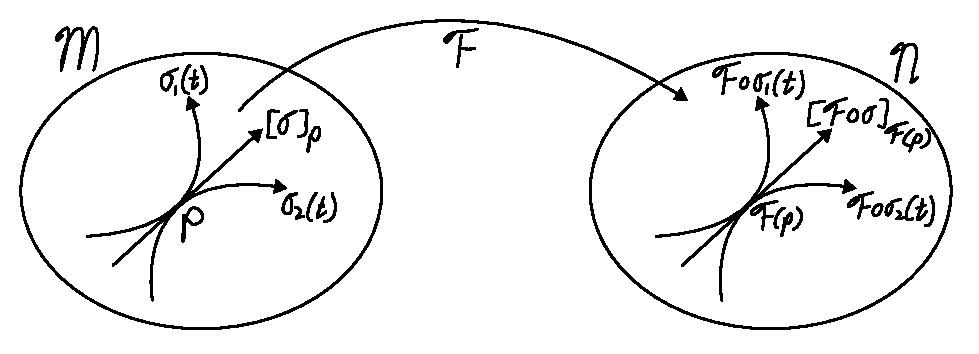
\includegraphics[width=0.7\textwidth, trim={0cm 0cm 0cm 0cm},clip]{push forward map}
      \caption[]{The push forward of an equivalence class of curves
      $[\sigma]_p$ induced by the map $\mathcal{F}$.}
      \label{fig: push forward map}
    \end{figure}
    \subsection{Calculating a push-forward of a tangent vector}
      \label{subsec: calculating a push-forward of a tangent vector}
      From definition~\ref{defn: push-forward defn}, we have
      \[\mathcal{F}_{*}(V_p^\sigma) = [\mathcal{F} \circ
      \sigma]_{\mathcal{F}(p)} = W^{\sigma^\prime}_{\mathcal{F}(p)}\]
      where $W^{\sigma^\prime}_{\mathcal{F}(p)} \in
      T_{\mathcal{F}(p)}(\mathcal{M})$. Now, for all $f \in
      C^k(\mathcal{N})$,
      \begin{align}
        W^{\sigma^\prime}_{\mathcal{F}(p)}(f) &=
        \left[\mathcal{F}_{*}(V_p^\sigma)\right](f) \nonumber \\
        &=\frac{d}{dt}\big[\mspace{-10mu}\underbrace{f \circ
        \mathcal{F}}_{\substack{\equiv f^\prime, \\
          f^\prime\in C^k(\mathcal{M})}} \mspace{-9mu} \circ\,
        \sigma\big](t)\Bigr|_{t = 0} \nonumber \\
        &= \frac{d}{dt}\big[f^\prime \circ \sigma \big](t)\Bigr|_{t = 0}\nonumber \\
        &= V^\sigma_p(f^\prime) \nonumber \\
        &= V^\sigma_p(f \circ \mathcal{F}) \label{eqn: important push forward result}
      \end{align}
    Now, in local charts $(U,\phi)$ and $(V,\psi)$ for $\mathcal{M}$ and
    $\mathcal{N}$ respectively, where for $p \in \mathcal{M}$ we define
    $\phi(p) \equiv x$ and $\psi(\mathcal{F}(p)) \equiv y$,
    equation~\ref{eqn: important push forward result} just reduces to:
    \begin{gather}
      % \label{eqn: push forward local chart}
      \left( W^{\sigma^\prime}_{\mathcal{F}(p)} \right)^i
      \left(\frac{\bar{f}(\mathcal{F}(p))}{\partial y^i}\right) =
      \left(V_p^\sigma\right)^i\left(\frac{\bar{f}(\mathcal{F}(p))}{\partial
      x^i}\right) \label{eqn: push forward local chart part 1} \\
      \implies \left( W^{\sigma^\prime}_{\mathcal{F}(p)} \right)^i
      \left(\frac{\partial \bar{f}(y^1,...,y^m)}{\partial y^i}\right) =
      \left(V_p^\sigma\right)^i\left(\frac{\partial \bar{f}(y^1(x^1,...,x^m),...,y^m(x^1,...,x^m))}{\partial
      x^i}\right)
    \end{gather}
    where $\bar{f} = f \circ \psi^{-1}$. This finally gives us:
    \begin{equation}
      \label{eqn: push forward local chart part 3}
      \left( W^{\sigma^\prime}_{\mathcal{F}(p)} \right)^i
      \left(\frac{\partial \bar{f}(y^1,...,y^m)}{\partial y^i}\right) =
      \left(V_p^\sigma\right)^i \frac{\partial y^j}{\partial x^i}
      \left(\frac{\partial \bar{f}(y^1,...,y^m)}{\partial y^j}\right)
    \end{equation}
    The detailed working to fully derive equation~\ref{eqn: push forward
    local chart part 3} is done in the context of fields in
    corollary~\ref{corollary: f-related field calculation}, but the working
    in corollary~\ref{corollary: f-related field calculation} can be easily
    adapted to quickly properly derive equation~\ref{eqn: push forward
    local chart part 3}.

    The hope is that the reader can see equation~\ref{eqn: push forward
    local chart part 1} as intuitive from equation~\ref{eqn: important push
    forward result} (if not, stare at it until it becomes intuitive).
    
    We will use the calculation here when we talk about
    $\mathcal{F}$-related vector fields in section~\ref{sec: mapping
    of vector fields} to derive some cool results for vector fields.
  \subsection{Push forward map induced by a curve}
    \label{subsec: push forward induced by a curve}
    Recall that a curve $\sigma$ on a manifold is an injective map from $I
    \subset \mathbb{R} \rightarrow \mathcal{M}$. Now, we can treat $I
    \subset \mathbb{R}$ as an open set of the one-dimensional manifold
    $\mathbb{R}$. This manifold, which admits a global chart, has a one
    dimensional tangent space $T_s(\mathbb{R})$ for all $s \in \mathbb{R}$.
    We can characterise the basis vector of the tangent space as
    $\frac{d}{dt}\Bigr|_{t=s}$ (here the coordinates of the manifold are
    labelled by $t$).

    Then, a tangent vector on $\mathcal{M}$ at the point $p = \sigma(s)$
    can be defined as the push forward of the tangent vector $\frac{d}{dt}\Bigr|_{t=s}$ induced by $\sigma$. I.e,
    \begin{equation}
      \sigma_{*}\left(\frac{d}{dt}\right)_{t = s} = V_{\sigma(s)} \in
      T_{\sigma(s)}(\mathcal{M})
    \end{equation}
    We will see this again when we talk about integral curves in
    section~\ref{sec: integral curves}.
  \subsection{Push forward map induced by a homeomorphism to
  $\mathbb{R}^m$}
    \label{subsec: push forward map induced by a homeomorphism}
    At a point $p \in \mathcal{M}$, under a local chart $(U,\phi)$, we
    recall that $T_p(\mathcal{M})$ has a coordinate basis
    $\left\{\frac{\partial}{\partial x^i}\right\}_{i = 1,...,m}$. Then, the
    map $\phi^{-1}$ induces a push-forward map between the coordinate basis
    in the local chart, and the actual basis vectors of $T_p(\mathcal{M})$,
    which we denote as: $\left\{e_i\right\}_{i = 1,...,m}$.